\chapter{Clang Analysis}

\section{Introduction}

In this chapter it will be described the analysis process and the tools used.\newline\newline
\textbf{Understand} is indeed the tool that gives the most accurate results in terms of checks, since it incorporates C/C++ MISRA standards, a beta version of the \textbf{Clang Static Analyzer}, which is a static analysis tool provided by the LLVM developers, and many other quality checks offered by SciTools itself.\newline
A simpler but also quite effective tool is \textbf{Cppcheck} which is designed to "provide unique code analysis to detect bugs and to focus on detecting undefined behaviour and dangerous coding constructs" \cite{bibitem2}. Also, as pointed by the developers, its main focus is to  "detect only real errors in the code (i.e. have very few false positives)". Cppcheck refers to the \textsl{Common Weakness Enumeration} standard for the analysis, a formal list of quality and security issues published by the MITRE institute. It is also possible to check MISRA-C project compliance but it requires to buy the standard so this feature was not used. \newline
The last used tool is \textbf{Flawfinder} which puts its focus more on security flaws rather than quality issues. This tool incorporates an option to run the analysis in order to detect possible false positives in an automated manner. This tools uses the CWE standard as Cppcheck does.\newline
Other tools such as \textbf{SonarQube} and \textbf{Cert C Rosechecker} were used but due to their characteristics they were unusable for our purpose.
\pagebreak

\section{Analysis Methodology}

The LLVM Clang compiler was analized with all the tools listed above.\newline
Since there were some technical problems while analyzing the whole project, as it was pointed in the previous section, a representative subset of it was chosen. In particular the folder \textbf{src/tools/libclang} was analyzed because it has been observed that the source files in this folder contained much of the compiler logic. This was the input folder for all the static analysis tools.\newline\newline
After the output was produced, the second phase of the analysis could start. Since the output format of the various tool is hetherogenous, it was necessary to convert them in files of the same format: data were imported in Excel sheets in order to collect evidences about what files were the most vulnerable/contained more bugs and what kind of bugs/quality issues were the most common.

\section{Understand}

Understand is a very powerful tool for static analysis that can be used to analyze software written in multiple languages suchs as Java, Ada, Cobol, Python, C/C++\dots
Among the tools used, it is the only one that comes with a nice and user-friendly user interface that allows users to browse the analysis results with different views.

\subsection{Understand Project}

First of all, it must be created an \textsl{Understand Project}. In this first step you are asked to select the language of the software (C/C++ in our case study) and the directories/source files to be analyzed.\newline\newline
\vspace{1cm}
\begin{minipage}{\linewidth}
	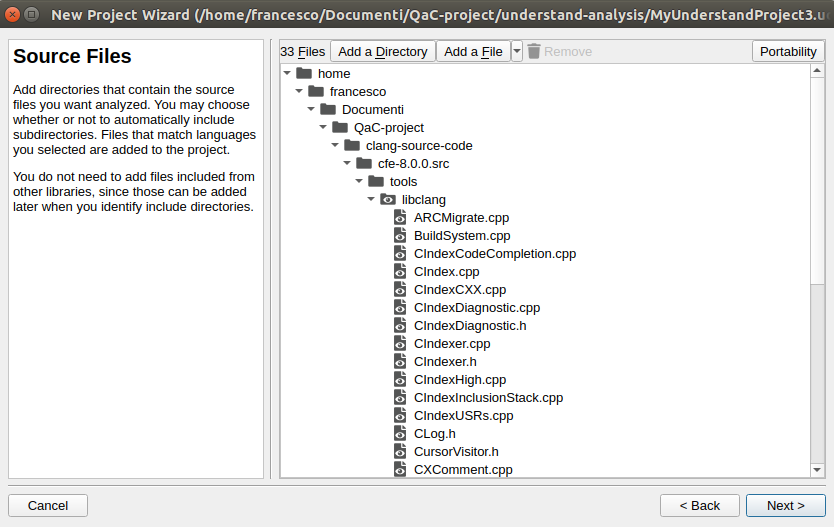
\includegraphics[width=\textwidth]{img/libclangDirectory.png}
	\captionof{figure}{The whole subdirectory tools/libclang is imported in the Understand project in order to run the analysis.}
\end{minipage}

When the files are loaded in the program, the analysis can be run simply by opening the \textsl{codecheck perspective} and selecting which standard should guide it.\newline\newline
\vspace{1cm}
\begin{minipage}{\linewidth}
	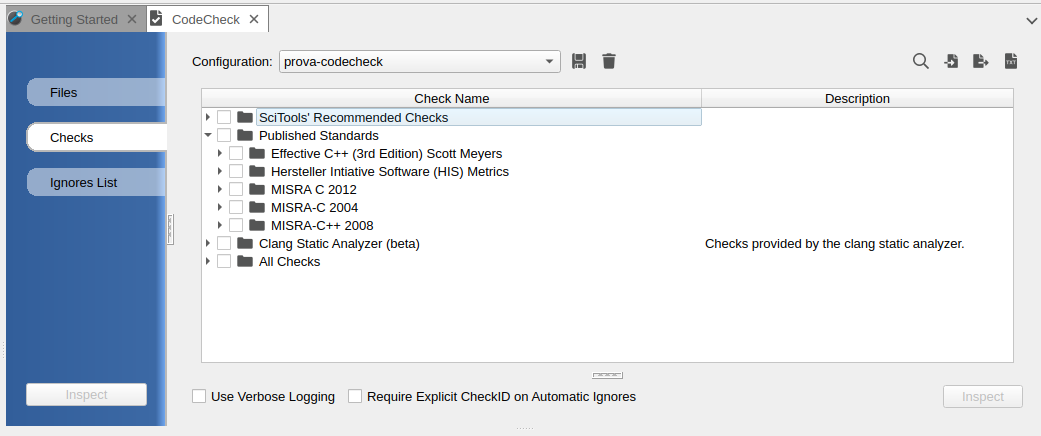
\includegraphics[width=\textwidth]{img/Codecheck.png}
	\captionof{figure}{The MISRA standard is incorporated in Understand, as well as the Clang Static Analyzer. Generic checks are also offered by the tool as \textsl{SciTools Recommended Checks} and \textsl{AllChecks}, some of which are redundant.}
\end{minipage}

\begin{itemize}
	\item \textsl{SciTools' Recommended Checks} - This is a small set (17 items) of generic good programming rules
	\item \textsl{Published Standards} - This section contains the published standards supported by Understand
		\begin{itemize}
			\item It was used the MISRA-C++ 2008 due to the nature of the source files (.cpp) and because one of the goals of this project was to check the Clang compiler compliance to MISRA rules
		\end{itemize}
	\item \textsl{Clang Static Analyzer} - It's an implementation of the Clang Static Analyzer tool, included in Understand
	\item \textsl{All Checks} - This is a collection of checks which consists of generic good programming rules and some of the MISRA rules. Despite its name, not all the checks are included for real, this is the reason why it's incorrect to use only this option for a consistent analysis
\end{itemize}

\subsection{Understand Output Format}

When the analysis ends, it is possible to navigate through different perspectives of what has been observed. For example it is possible to list results \textsl{by file}, in order to check what issues are present in each file (and at which line of code) and what files contain the most issues. Another possibility is to display results \textsl{by check}, that is: for each rule (e.g. MISRA) how many times it has been violated and where (in terms of files).\newline
Two very interesting features offered by Understand are the:
\begin{itemize}
	\item Result Locator
	\item Result Treemap
\end{itemize}

The first offers the possibility to navigate through the findings, filtering them by file, by violation and some other options, giving the possibility to jump to the desired \textsl{vulnerable} line of code in the source file.\newline
The result treemap instead gives you a graphic representation of the vulnerabilities found in the files, in terms of criticity and quantity. These characteristics can be viewed graphically using colored boxes, where the meaning of the color/dimension of the boxes can be defined by the user.\newline
Mastering the options of these two powerful features gives to the user much more control of the analysis and a wider perspective of the whole project quality.\newline\newline

\vspace{1cm}
\begin{minipage}{\linewidth}
	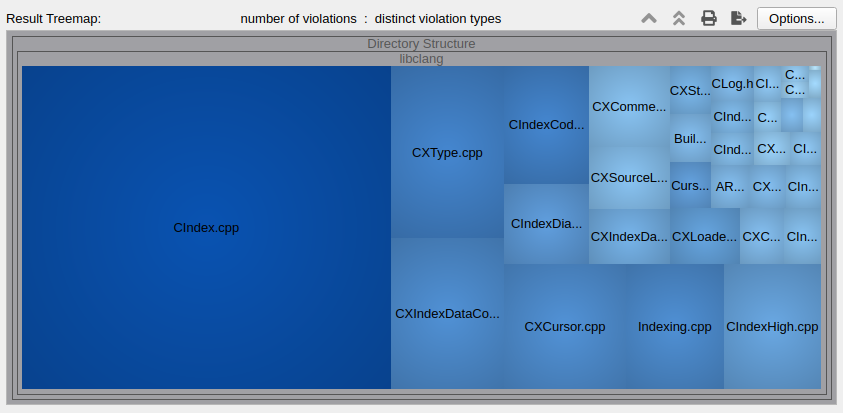
\includegraphics[width=\textwidth]{img/AllChecksTreeMap.png}
	\captionof{figure}{Result Treemap view.}
\end{minipage}
\vspace{1cm}

All the output perspectives can be exported in suitable formats (e.g. Treemap is exported in .png files while lists of violations are exported in .txt or .html files) that facilitated the second phase of the analysis.

\subsection{Understand Results}

As it has been said in the introduction, multiple analyses with different checks were run:
\begin{itemize}
	\item[$a)$] MISRA-C++ 2008
	\item[$b)$] SciTools' Recommended Checks
	\item[$c)$] All Checks
	\item[$d)$] Clang Static Analyzer
\end{itemize}

\hspace{-0.6cm} \textbf{$a)$}  
This check is based on the MISRA-C++ 2008 standard, which is a standard developed for the quality check of C++ source files.\newline
Results have been sorted by file and by MISRA rule. After that a compact view of these was produced showing the amount of violations for each MISRA and for each file.\newline
Analyzing the reports it can be observed that:
\begin{itemize}
	\item The total number of violations in the \textbf{libclang} folder is 8450
	\item The first three rules that were violated the most are:
	\begin{itemize}
		\item[$1.\:$] MISRA08\_7-1-1 - \textbf{A variable which is not modified shall be const qualified} - 1845 violations.\newline If a variable does not need to be modified, then it shall be declared with const qualification so that it cannot be modified. A non-parametric variable will then require its initialization at the point of declaration. Also, future maintenance cannot accidentally modify the value
		\item[$2.\:$] MISRA08\_6-4-1 - \textbf{An if condition construct shall be followed by a compund statement. The else keyword shall be followed by either a compound statement or another if statement} - 1239 violations.\newline If the bodies of these constructs are not compound statements, then errors can occur if a developer fails to add the required braces when attempting to change a single statement body to a multistatement body. Requiring that the body of these constructs shall be a compound statement (enclosed within braces) ensures that these errors cannot arise
		\item[$3.\:$] MISRA08\_0-1-10 -\textbf{All defined functions called} - 733 violations.\newline Functions or procedures that are not called may be symptomatic of a serious problem, such as missing paths
	\end{itemize}
	\item The first three files that contain the most violations are:
		\begin{itemize}
		\item[$1.\:$] CIndex.cpp - 3828 violations
		\item[$2.\:$] CXType.cpp - 757 violations
		\item[$3.\:$] CXCursor.cpp - 558 violations
	\end{itemize}
\end{itemize}

Looking at the complete report, considerations can be made on the following aspects:

\begin{itemize}
	\item Some of the violations found (e.g. MISRA08\_0-1-10) include for sure some false-positive, due to the fact that the analysis was performed on a small subset of the complete project. Maybe the violation count for these rules could be reduced by performing a more comprehensive analysis
	\item The violations distribution is reasonable, that is that most of the files have a similar issues count and the same can be said for MISRA rules
	\item There is an exception both for files and for MISRA:
	\begin{itemize}
		\item[FILE: ] CIndex.cpp (3828 violations wrt 8450 total violations)
		\item[MISRA: ] MISRA08\_7-1-1 (1845 violations wrt 8450 total violations)
	\end{itemize}
	\item Using the Result Treemap feature it is possible to observe that the $NumberOfViolations/CountLineCode$ ratio varies between [0.27 - 1.75]
	\item Combining the use of the Result Treemap and Result Locator it is observable that the first 3 files in terms of $NumberOfViolations/CountLineCode$ ratio are relatively small files compared to the others
	
\end{itemize}

\vspace{1cm}

\begin{minipage}{\linewidth}
	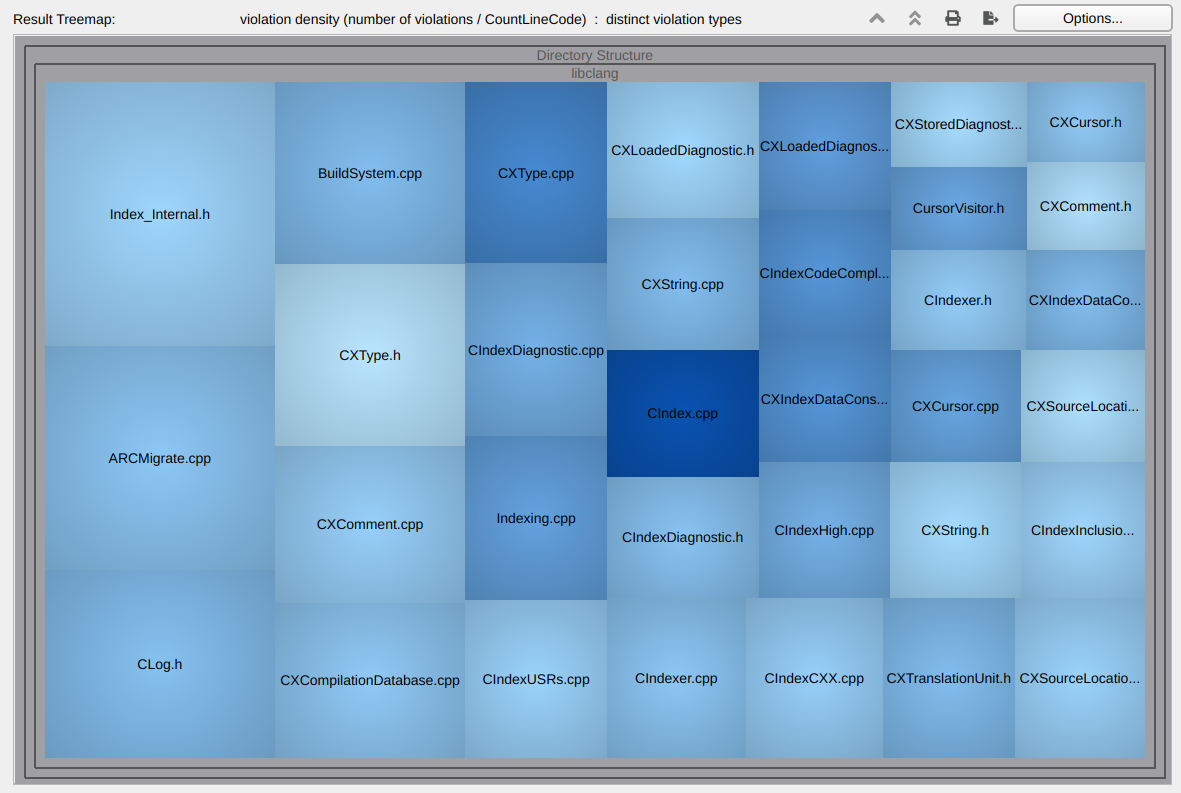
\includegraphics[width=\textwidth]{img/TreemapCountLine.png}
	\captionof{figure}{Result Treemap where files are sorted by $NumberOfViolations/CountLineCode$ ratio. Darker boxes indicates more distinct violation types while wider boxes indicate higher ratio.}
\end{minipage}
\pagebreak

\hspace{-0.6cm} \textbf{$b)$}  
SciTools Recommended Checks is a set of 17 quality checks based on code quality conventions that does not follow any precise standard.\newline
Results has been sorted by files and by the checkID provided by Understand. The postprocess phase was very similar to the previous one in order to obtain a compact view of data.\newline

\begin{itemize}
	\item The total number of violations in the \textbf{libclang} folder is 3299 (roughly 1000 violations less than the MISRA-check).
	\item The first three checks that were violated the most are:
	\begin{itemize}
		\item[$1.\:$] RECOMMENDED\_16 - \textbf{Each variable declaration should have a comment} - 1774 violations.\newline
		\item[$2.\:$] RECOMMENDED\_13 - \textbf{Every defined function shall be called at least once} - 733 violations.\newline 
		\item[$3.\:$] RECOMMENDED\_08 -\textbf{All fixed values will be defined constants} - 405 violations.\newline
	\end{itemize}
	\item The first three files that contains the most violations are:
		\begin{itemize}
		\item[$1.\:$] CIndex.cpp - 1472 violations.
		\item[$2.\:$] CXType.cpp - 266 violations.
		\item[$3.\:$] CXCursor.cpp - 250 violations.
	\end{itemize}
\end{itemize}

As it can be noticed by these data, the three files that have the most violations are the same as in the MISRA analysis.\newline
Looking at the complete dataset and comparing it to the previous one, the following considerations can be made:
\begin{itemize}
	\item The \textsl{RECOMMENDED\_13} plays a similar role as the MISRA08\_0-1-10. We can expect that when the analysis runs on the whole project the count number of this violation (\textsl{Every defined function shall be called at least once}) drops.
	\item The \textsl{RECOMMENDED\_16} check may seem too exaggerated but, if we think to big project as LLVM-Clang is, where multiple teams cooperate writing different chunks of code, this check become reasonable.
	\item The violations distribution with respect to files is quite odd. It can be observed that the average of the violations count is approximately 100. If we exclude the CIndex.cpp file the average drops approximately to 55.
	\item There is an exception both for files and for check, as we saw in the previous section:
	\begin{itemize}
		\item[FILE: ] CIndex.cpp (1472 violations wrt 3299 total violations)
		\item[MISRA: ] RECOMMENDED\_16(1774 violations wrt 3299 total violations)
	\end{itemize}
	\item Using the Result Treemap feature it is possible to observe that the $NumberOfViolations/CountLineCode$ ratio varies between [0.09 - 0.39].
\end{itemize}

\vspace{1cm}
\begin{minipage}{\linewidth}
	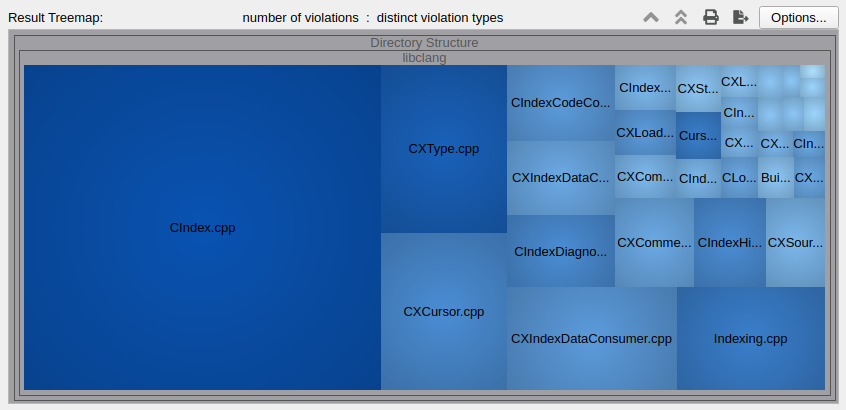
\includegraphics[width=\textwidth]{img/SciToolsViolationsCount.png}
	\captionof{figure}{Result Treemap where files are sorted by $NumberOfViolations$. As you can see the file CIndex.cpp covers almost half of the area.}
\end{minipage}
\pagebreak

\begin{minipage}{\linewidth}
	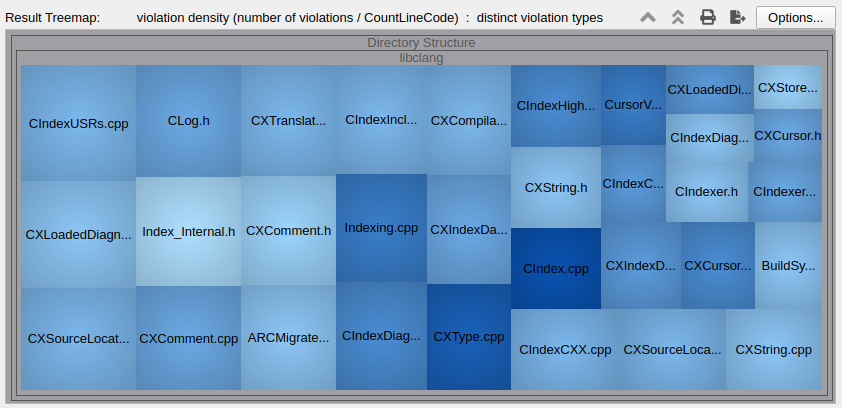
\includegraphics[width=\textwidth]{img/SciToolsViolationsRatio.png}
	\captionof{figure}{Despite the result in the previous figure, the $NumberOfViolations/LineOfCode$ ratio is quite homogeneous.}
\end{minipage}

\pagebreak

\hspace{-0.6cm} \textbf{$c)$}  
The \textsl{AllChecks} check set is the biggest among the provided ones. It includes most of the checks already seen in the previous sections, plus some completely new checks.\newline
Results has been sorted by files and by the checkID provided by Understand. The postprocess phase was very similar to the previous one in order to obtain a compact view of data.\newline

\begin{itemize}
	\item The total number of violations in the \textbf{libclang} folder is 30604 (indeed a very huge number compared to the previous ones).
	\item The first three checks that were violated the most are:
	\begin{itemize}
		\item[$1.\:$] CPP\_L000 - \textbf{Calls to COTS (Commercial Off The Shelf) library functions that might throw an exception, must be enclosed in a try block} - 5921 violations.\newline
		\item[$2.\:$] CPP\_I005 - \textbf{Identifier name reuse} - This check is concerned about variables' names. It requires that, in the same file, a different name is given to every different variable - 3546 violations.\newline 
		\item[$3.\:$] CPP\_V006 -\textbf{A variable which is not modified should be const qualified} - same as MISRA analysis - 1845 violations.\newline
	\end{itemize}
	\item The first three files that contains the most violations are:
		\begin{itemize}
		\item[$1.\:$] CIndex.cpp - 14004 violations.
		\item[$2.\:$] CXType.cpp - 2311 violations.
		\item[$3.\:$] CXIndexDataConsumer.cpp - 2078 violations.
	\end{itemize}
\end{itemize}

It is noticeable that, with this set of checks, the third file with most violations is \textsl{CXIndexDataConsumer.cpp} instead of \textsl{CIndex.cpp}.\newline
Let's now proceed with some considerations on this analysis as well:

\begin{itemize}
	\item Since this analysis include the previous ones, we assume that there are false-positives but they are caused mostly by the fact that the inspection was done on a subpart of the project. We don't have evidences of false-positives among the most common violations (see the complete excel report for more details).
	\item The most frequent violation is of a new kind. It is an important vulnerability that was pointed by none of the other analysis. This is quite odd since this is a quite important rule, well accepted by the developer community.
	\item The violations distribution with respect to files is similar to the previous ones.
	\item The violations distribution with respect to checks is almost uniformly distributed. This behaviour is gradually lost when the violations count goes over approximately 400)
	\item As well as the previous analysis, there is an exception both for files and for checks:
	\begin{itemize}
		\item[FILE: ] CIndex.cpp (14004 violations wrt 30604 total violations, almost half of the total)
		\item[MISRA: ] CPP\_L000(5921 violations wrt 30604 total violations. Recall that the second most common check had more than 2000 violations less)
	\end{itemize}
	\item Using the Result Treemap feature it is possible to observe that the $NumberOfViolations/CountLineCode$ ratio varies between [1 - 5.45]
\end{itemize}

\begin{minipage}{\linewidth}
	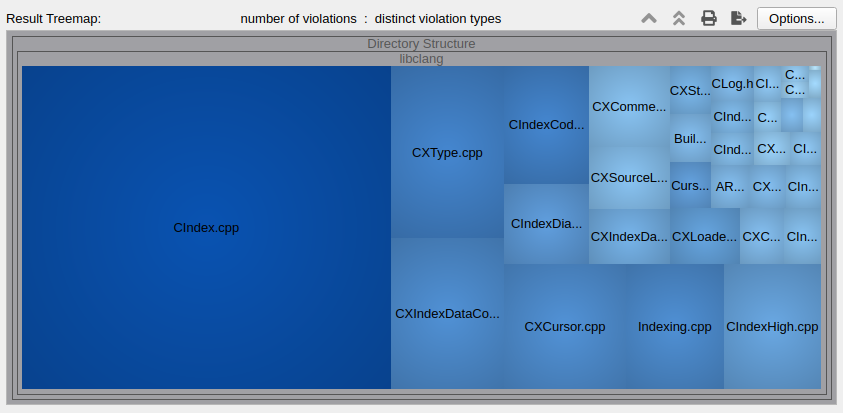
\includegraphics[width=\textwidth]{img/AllChecksTreeMap.png}
	\captionof{figure}{The CIndex.cpp file covers almost half of the total area also in this figure.}
\end{minipage}

\begin{minipage}{\linewidth}
	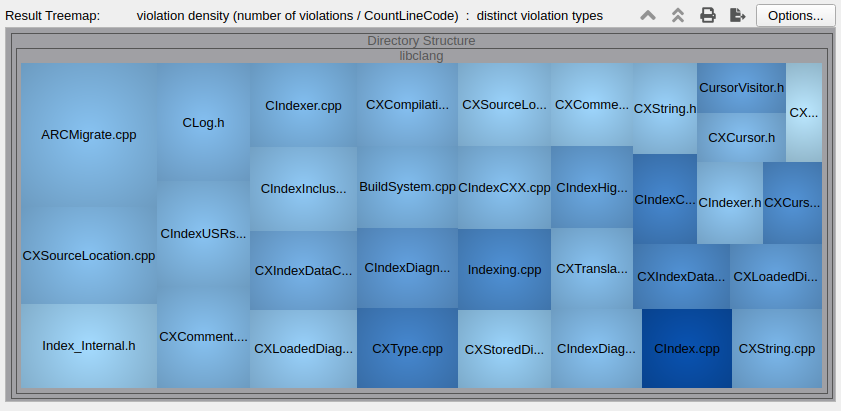
\includegraphics[width=\textwidth]{img/AllChecksViolationsRatio.png}
	\captionof{figure}{Even if the proportion of the $max/min$ of the ratio is similar to the previous, the ratio distribution itself is quite sparse (it ranges between 1 and 5.5), as well as the first analysis.}
\end{minipage}
\pagebreak

\hspace{-0.6cm} \textbf{$d)$}  
The \textsl{Clang Static Analyzer} check set is an implementation of the Clang Static Analyzer tool, developed as part of the LLVM-Clang project.\newline
The Clang Static Analyzer itself has not been used since it requires the build of the \textsl{whole} project to scan it. Moreover the increased knowledge of Understand and the presence of this set of checks embedded in the tool led us to the choice of using this implementation rather than the standalone tool.\newline\newline
This analysis did not find any violation. This seems reasonable since the metrics and quality practices chosen during the development of the LLVM-Clang compiler are probably the same metrics and checks implemented in the analyzer.

\subsection{Reports Summary}

In this conclusive section for the Understand analyzer, will be presented a summary of the most important observations along with some cross-checks. Summaries of the data collected throughout these analysis are reported at the end of the \textsl{Understand section}.\newline
\begin{itemize}

	\item All the analysis agreed that CIndex.cpp is the file with the largest violations count. The violations number of this file is usually very large, compared to the others.
	\item CXType.cpp is always the second file with the largest violations count. There are variations from the third position onwards, for example: CXCursor.cpp appears 2 times in the third position, while CXIndexDataConsumer.cpp appears 1 time.
	\item Looking at the $violationsCount/countLineCode$ ratio, it is observable that across the three analysis the $min/max$ proportion is very similar ($\approx 5.5 \pm 1$).
	\item It seems reasonable that using the metrics chosen by the project developers to analyze the source code no violations are found while, when different metrics are used, there are some violations.
	\item In some cases the violated metrics could be considered as a warning (e.g. to write a comment for every variable helps to keep the project well documented) while in some other cases (e.g. do not use try-catch construct) they are critical issues.
	\item Very likely, in these analyses, there are some false positives. This is because of the fact that the analyses were not performed on the whole project (e.g. functions that are never called in the analyzed modules could be called somewhere else).
	\item Some duplicated violations were reported when performing the analysis using the MISRA set. This is likely to be attributable to a possible overflow issue that has been noted also in the very first phase of the use of Understand. The duplicated issues had been removed in order to clean the dataset. No duplications were found using the other sets of rules.
\end{itemize}

\subsection{Understand Performances}

Understand is a very powerful tool, that comes with an easy-to-use user-interface and that gives a lot of informations about the performed analysis (e.g. result Treemap, result Locator, sort by check/file\dots)
On the other hand, it is not a lightweight program: we experienced unexpected crashes during analyses, issues duplication and a slow execution time in general. These are some of the main reasons that forced us to work on a subset of the LLVM-Clang compiler.\newline
Compared to the tools that will be presented in the next sections, this is indeed the most efficient in terms of \textsl{informations} and \textsl{versatility} (The various views it offers are a very powerful tool to navigate through the data). On the other hand, in terms of actual performance, it was the slowest one.

\pagebreak

\begin{minipage}{\linewidth}
	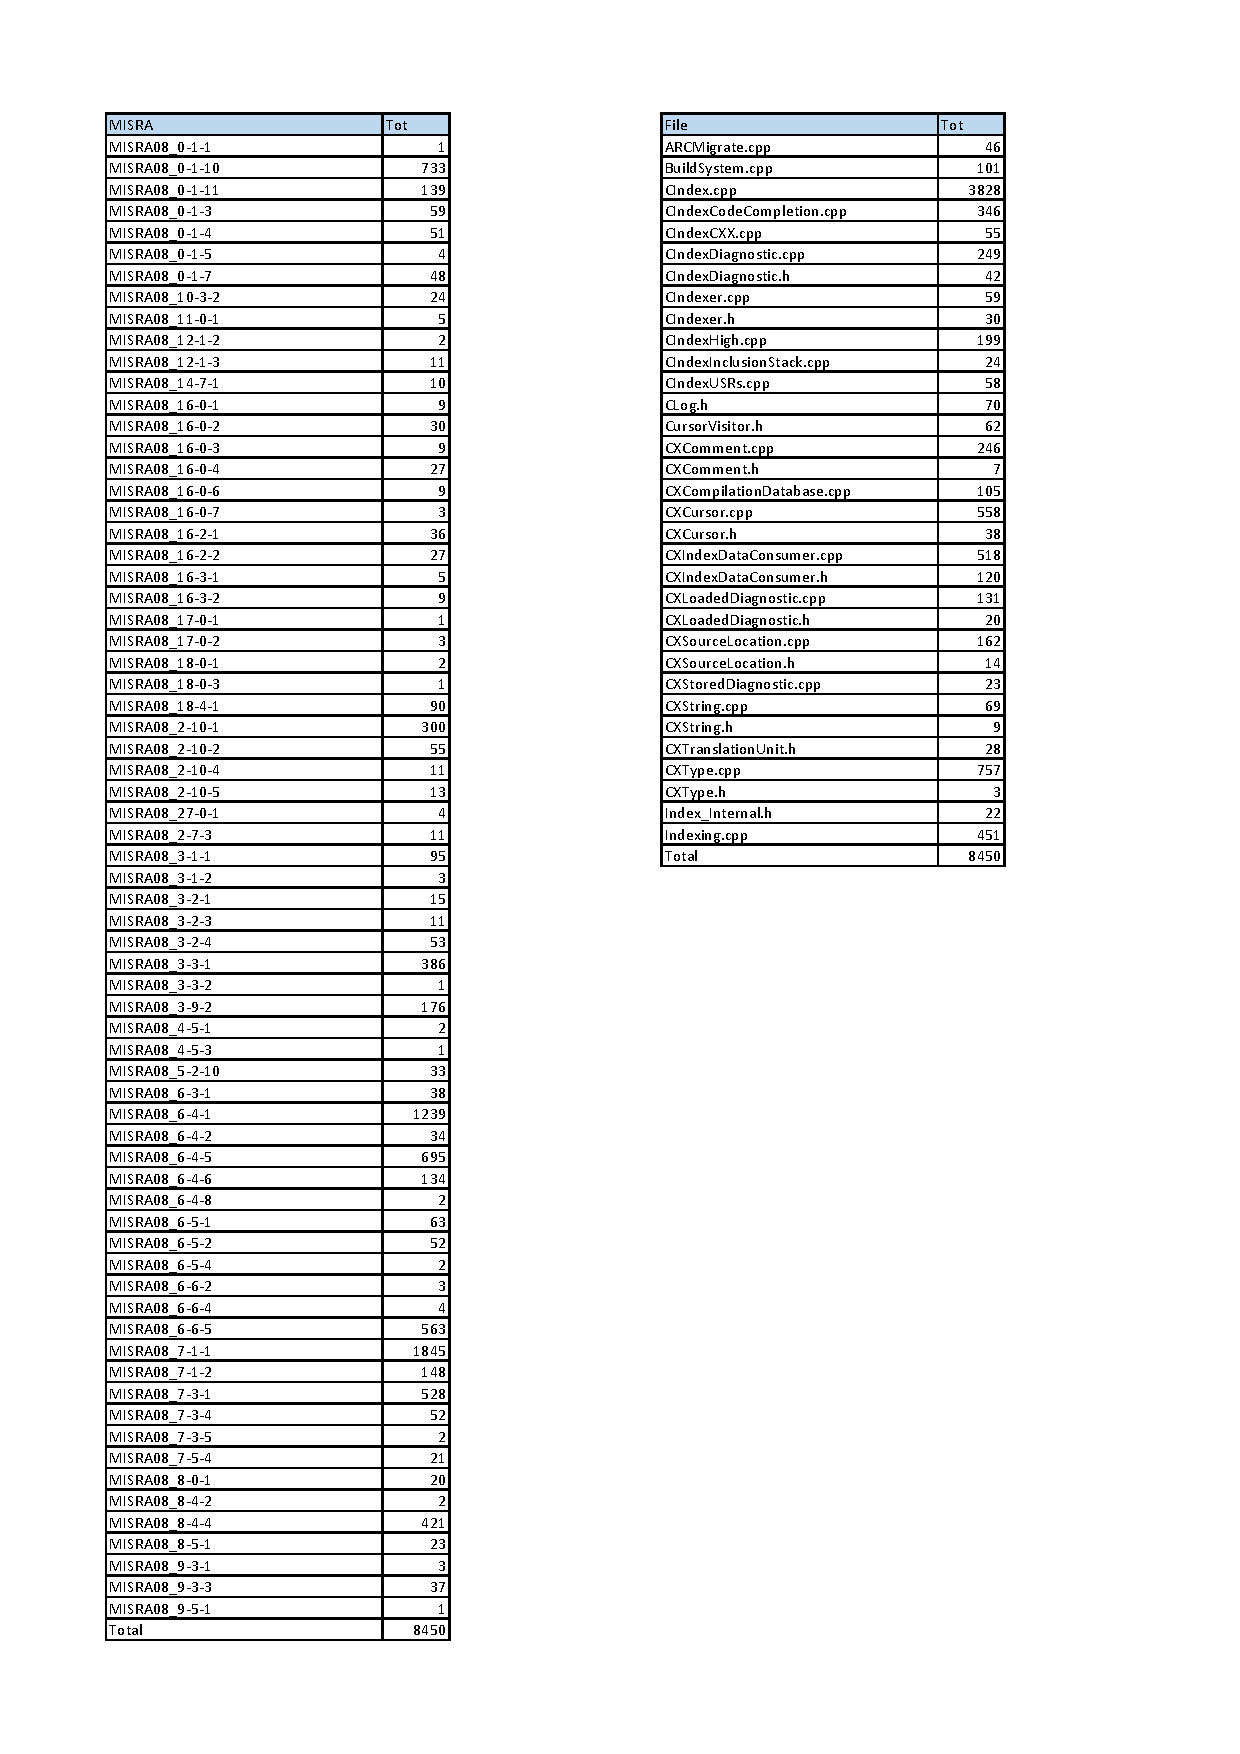
\includegraphics[width=\textwidth]{pdf/Misra_Summary.pdf}
	\captionof{figure}{Summary of the MISRA checks}
\end{minipage}

\pagebreak

\begin{minipage}{\linewidth}
	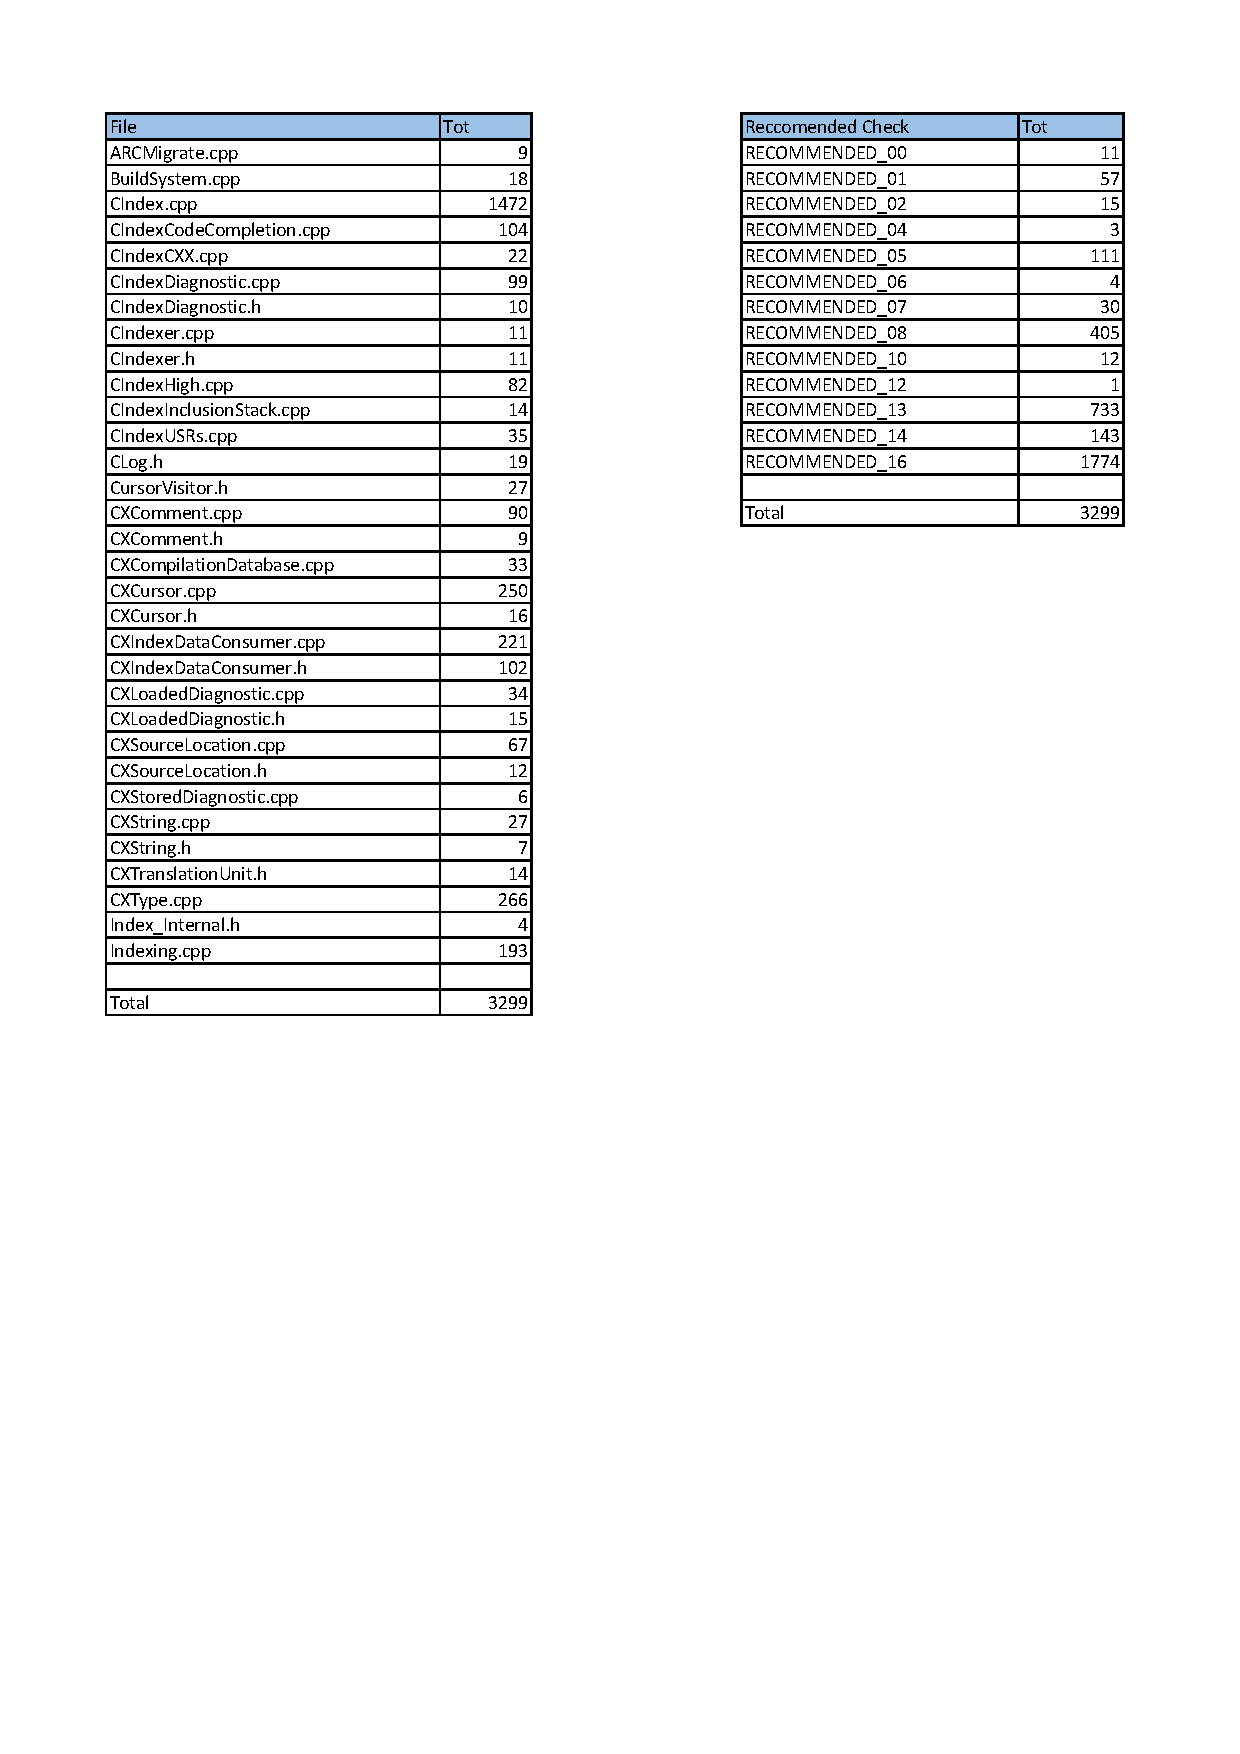
\includegraphics[width=\textwidth]{pdf/SciTools_Summary.pdf}
	\captionof{figure}{Summary of the SciTools Recommended Checks}
\end{minipage}

\pagebreak

\begin{minipage}{\linewidth}
	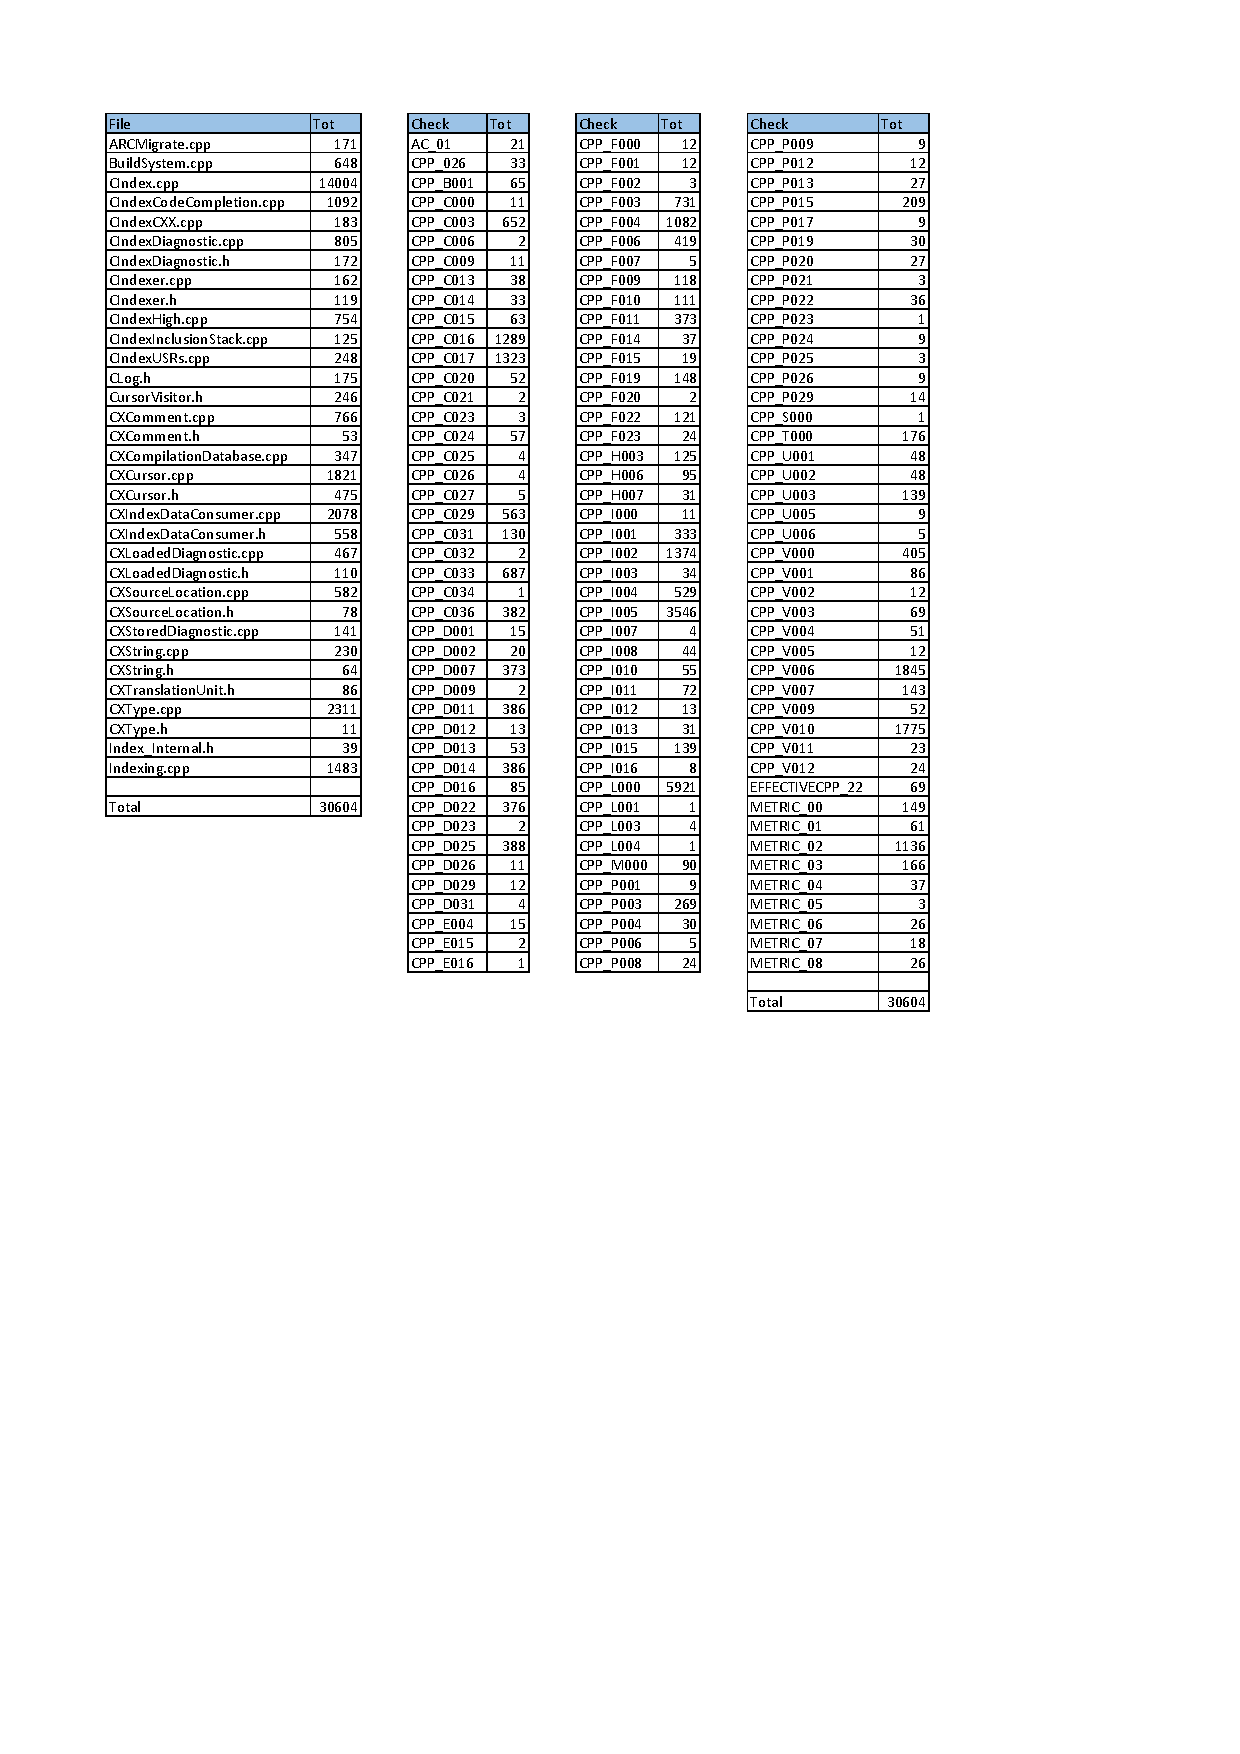
\includegraphics[width=\textwidth]{pdf/AllChecks_Summary.pdf}
	\captionof{figure}{Summary of the AllChecks checks}
\end{minipage}

\section{Cppcheck Analysis}

Cppcheck is a lightweight, open-source tool for static analysis of C/C++ files. It can be downloaded at \url{http://cppcheck.sourceforge.net} for Windows (an installer is provided), Mac and Linux distributions:
\begin{itemize}
	\item sudo apt-get install cppcheck (Linux)
	\item brew install cppcheck (Mac)
\end{itemize}
Once installed, the tool can be run via terminal using the following command:
\begin{itemize}
	\item cppcheck [OPTIONS] [files or directories]
\end{itemize}

The [OPTIONS] option offers some sort of customization of the analyses, for example it allows the user to:
\begin{itemize}
	\item Write results to an xml file
	\item Print the list of all the available checks
	\item Print the error list in xml format (on the console)
	\item Suppress specific warnings
	\item Define/undefine preprocessor symbol
	\item And more (see cppcheck --help for more informations)\dots
\end{itemize}
The analyzer can be fed with a single file, a list of files, or a whole directory. In this study, for compliance with the \textsl{Understand} analysis, the check was done on the \textbf{tools/libclang} directory.\newline
The output was written to an xml file and postprocessed with excel.

\subsection{Cppcheck Results}

Cppcheck relies on the MITRE-CWE list to detect vulnerabilities and quality issues, plus some generic quality checks based on standard code quality practices.\newline
The CWE list stands for Common Weakness Enumeration. It associate IDs to code issues categories that can be refined by users (e.g. it was not possible to find a 1:1 correspondence between the checkNames provided by Cppcheck and the checkNames provided in the CWE list, although the CWE IDs were identical).
\newline In this analysis were found issues related to four CWE categories:

\begin{itemize}
	\item[(CWE-398) ] \textbf{Code Quality} - This category represents one of the phyla in the Seven Pernicious Kingdoms vulnerability classification. It includes weaknesses that do not directly introduce a weakness or vulnerability, but indicate that the product has not been carefully developed or maintained. According to the authors of the Seven Pernicious Kingdoms, "Poor code quality leads to unpredictable behavior. From a user's perspective that often manifests itself as poor usability. For an adversary it provides an opportunity to stress the system in unexpected ways." \cite{bibitem3}.
	\item[(CWE-561) ] \textbf{Dead Code} - Dead code is source code that can never be executed in a running program. The surrounding code makes it impossible for a section of code to ever be executed \cite{bibitem4}.
	\item[(CWE-563) ] \textbf{Assignment to Variable without Use} - After the assignment, the variable is either assigned another value or goes out of scope. It is likely that the variable is simply vestigial, but it is also possible that the unused variable points out a bug \cite{bibitem5}. 
	\item[(CWE-686) ] \textbf{Function Call With Incorrect Argument Type} - This weakness is most likely to occur in loosely typed languages, or in strongly typed languages in which the types of variable arguments cannot be enforced at compilation time, or where there is implicit casting \cite{bibitem6}.
\end{itemize}

Moreover, Cppcheck rise a warning about missing files that are included in source cpp files but that are not found in the analyzed directory.\newline
This warning tells the user that the analysis will terminate but "results will probably be more accurate if all the include files are found".\newline\newline

Results have been sorted, as the previous analyses, by files and by the checkName provided by Cppcheck. Again, results were aggregated in excel files to ease data observation.\newline
Analyzing the reports it can be observed that:
\begin{itemize}
	\item The total number of violations in the \textbf{libclang} folder is 414 (very small number compared to e.g. MISRA violations)
	\item The first three rules that were violated the most are:
	\begin{itemize}
		\item[$1.\:$] CWE-561 - \textbf{Unused Function} - 375 violations.
		\item[$2.\:$] CWE-398 - \textbf{No explicit contructor} - 11 violations.
		\item[$3.\:$] CWE-398 -\textbf{Uninit Member Var} - 10 violations.
	\end{itemize}
	\item The first three files that contains the most violations are:
		\begin{itemize}
		\item[$1.\:$] CIndex.cpp - 158 violations.
		\item[$2.\:$] CXType.cpp - 47 violations.
		\item[$3.\:$] Indexing.cpp - 35 violations.
	\end{itemize}
\end{itemize}

\subsection{Cppcheck Performance \& Comparison with Understand}

Cppcheck is a much faster tool than Understand. The absence of UI and its simpleness play an important role on its performances: it works directly on the directories instead of creating a \textsl{project file} that acts as a link from the source files to the tools; on the other hand this simpleness provides less informations on the project issues.\newline
Cppcheck output is displayed on console only by default. Using a proper option it is possible to write the outputs to an xml file, reducing its readibility.\newline
Comparing it to Understand, it has been seen that, in this study, Cppcheck did not produced any duplicate issue (same file, same issue, same line of code).\newline\newline

We now present some comparison of the results achieved with Understand and the ones obtained by Cppcheck.\newline
First of all the issues count distribution for checks and files is almost uniformly distributed, at least compared to the MISRA-checks, although there is always the exception of the false positive \textsl{unused functions} and the \textsl{CIndex.cpp} file, which is the biggest file in the directory (therefore it contains much more violations with respect to the others).\newline\newline
Some of the Cppcheck CWE-checks are overlapping with the MISRA checks. The "duplicated" issues that were found are:

\begin{itemize}
	\item \textbf{MISRA08\_12-1-3} - All constructors that are callabe with a single argument of fundamental type shall be declared explicit - 11 violations
	\item \textbf{Cppcheck CWE-398} - No Explicit Constructor - 11 violations
\end{itemize}

These 2 checks refer to a quality practice in which constructors with a single argument should be declared \textsl{explicit}. The MISRA check indeed provides much more informations than the Cppcheck check.\newline
It is noticeable that both the tools find the same amount of violations for this check.

\begin{itemize}
	\item \textbf{MISRA08\_0-1-3} - A project shall not contain unused variables - 59 violations
	\item \textbf{Cppcheck CWE-563} - Unred variable - 1 violation
\end{itemize}

The MISRA check is more general, compared to the Cppcheck. This one refers only to variables that are never read, while the MISRA check refers to variables that are declared but never used in general. There is a huge difference on the amount of violations found: 59 for the MISRA, 1 for Cppcheck.

\begin{itemize}
	\item \textbf{MISRA08\_8-5-1} - All variables shall have a defined value before they are used - 23 violations
	\item \textbf{Cppcheck CWE-398} - Uninit Member Var - 10 violations
\end{itemize}

Cppcheck reported a large amount of "Unused Functions" (375 violations on 414 totally found) and, as for Understand where 733 violations of this kind were found with the MISRA set of rules, we suppose that this could be caused by the fact that not the whole project has been analyzed.\newline
It is odd that the $UnusedFunctions/TotalViolations$ proportion changes this much: $90\%$ (Cppcheck) versus $9\%$ (Understand).\newline
Generally speaking Cppcheck reported less issues than Understand.
\pagebreak

\begin{minipage}{\linewidth}
	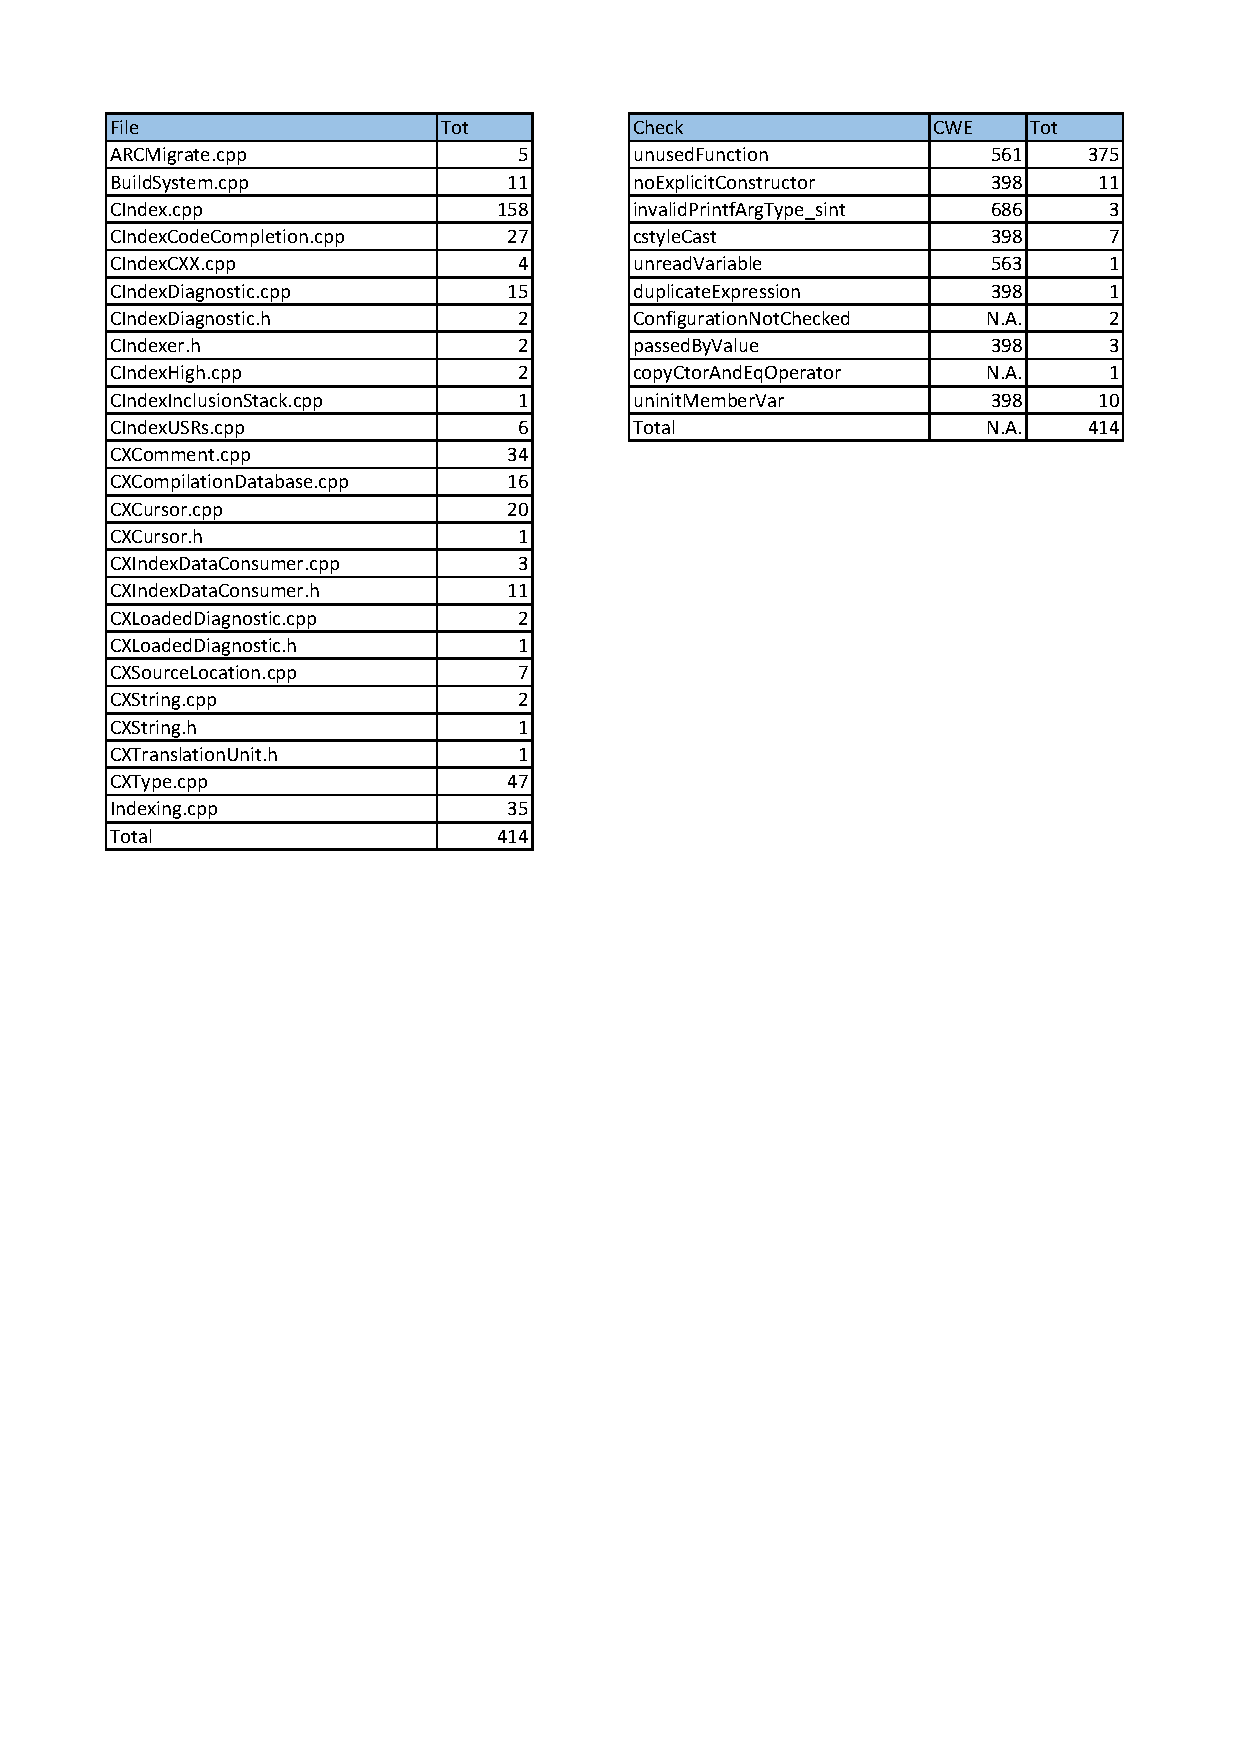
\includegraphics[width=\textwidth]{pdf/Cppcheck_Summary.pdf}
	\captionof{figure}{Summary of the Cppcheck checks}
\end{minipage}

\section{Flawfinder Analysis}

Flawfinder has the same charachteristics as Cppcheck. It is a light (runnable from console, without UI) and open-source.\newline
The big difference with the previous tools is that Flawfinder is designed to find vulnerabilities more related to \textsl{computer security} rather than code quality issues and bugs.\newline
It can be downloaded at \url{https://dwheeler.com/flawfinder/#downloading}.\newline
Once installed, the tool can be run via terminal using the following command:
\begin{itemize}
	\item flawfinder [OPTIONS] [files or directories]
\end{itemize}

Flawfinder has much more [OPTIONS] than Cppcheck, for example:\begin{itemize}
	\item Write results to a txt, csv or html file
	\item Ignore specific files
	\item Set the minimum risk level to be included in the \textsl{hit list}
	\item Display hits without waiting for the end of the analysis
	\item An option to don't include false positive. This option was used for one analysis but, as pointed in the documentation, this is risky since it does not follow any standard procedure to exclude likely false positives. For this reason, results found using this options were not considered to be trustable.
	\item And more (see flawfinder --help for more informations)\dots
\end{itemize}

As with the previous tools, Flawfinder performed its analyses on the \textbf{tools/libclang} directory.

\subsection{Flawfinder Results}

The checks performed by Flawfinder are based on the MITRE-CWE list as well as Cppcheck.\newline
The issues categories found during the analyses are listed below:

\begin{itemize}
	\item[(CWE-20) ] \textbf{Improper Input Validation} - When software does not validate input properly, an attacker is able to craft the input in a form that is not expected by the rest of the application. This will lead to parts of the system receiving unintended input, which may result in altered control flow, arbitrary control of a resource, or arbitrary code execution \cite{bibitem7}.
	\item[(CWE-120) ] \textbf{Buffer Copy without Checking Size of Input} - A buffer overflow condition exists when a program attempts to put more data in a buffer than it can hold, or when a program attempts to put data in a memory area outside of the boundaries of a buffer. The simplest type of error, and the most common cause of buffer overflows, is the "classic" case in which the program copies the buffer without restricting how much is copied. Other variants exist, but the existence of a classic overflow strongly suggests that the programmer is not considering even the most basic of security protections \cite{bibitem8}.
	\item[(CWE-807) ] \textbf{Reliance on Untrusted Inputs in a Security Decision} - Developers may assume that inputs such as cookies, environment variables, and hidden form fields cannot be modified. However, an attacker could change these inputs using customized clients or other attacks. This change might not be detected. When security decisions such as authentication and authorization are made based on the values of these inputs, attackers can bypass the security of the software.\newline
Without sufficient encryption, integrity checking, or other mechanism, any input that originates from an outsider cannot be trusted \cite{bibitem9}.
\end{itemize}

Some of the issues found by Flawfinder are tagged with the tag: [MS-banned]. This tag refers to particular functions that are in the \textsl{banned functions list} published by Microsoft \cite{bibitem10}. These are functions that contains critical and well-known security vulnerabilities such, e.g. \textsl{strcpy} that introduces a \textsl{buffer overflow} vulnerability.\newline\newline

Comparing the issues found with the previous reports, Flawfinder found a small number of vulnerabilities, this is also caused by the fact that this tool only looks for security issues.\newline
The total vulnerability count is 32, distributed in the 3 CWE categories listed above.\newline
The top three vulnerabilities are:
	\begin{itemize}
		\item[$1.\:$] CWE-807, CWE-20 - Environment variables are untrustable input if they can be set by an attacker. They can have any content and length, and the same variable can be set more than once - 17 violations.
		\item[$2.\:$] CWE-120 - Does not check for buffer overflows when copying to destination - 6 violations.
		\item[$3.\:$] CWE-120 \textbf{[MS-banned]} - \textsl{strncpy} easily used incorrectly; doesn't always $\backslash0$-terminate or check for invalid pointers - 5 violations.
	\end{itemize}

And the top three files are:

\begin{itemize}
		\item[$1.\:$] CIndex.cpp - 14 violations.
		\item[$2.\:$] CIndexCodeCompletion.cpp - 6 violations.
		\item[$3.\:$] CIndexer.cpp \& Indexing.cpp - 3 violations. 
\end{itemize}

The number of violations found is very small so the only things that are noticeable are that:
\begin{itemize}
		\item CIndex.cpp also in this analysis is the file that contains the biggest amount of violations.
		\item Differing from the other analyses, Flawfinder found vulnerabilities only on 8 files out of 33.
		\item The most common causes of vulnerabilities found in this project are related to the use of environmental variables (17 violations out of 32) and the possible arise of buffer overflows (14 violations out of 32, combining different CWE checks).
\end{itemize}

Flawfinder offers an option to run the analysis without including possible false positives.\newline
As already said in the beginning of this section, results found with this options are not accurate. In particular, it has been reported that the possible false positive is:

\begin{itemize}
	\item[(CWE-119/120) ] Statically-sized arrays can be improperly restricted, leading to potential overflows or other issues.
\end{itemize}

This clearly isn't a false positive since this is a well-known vulnerability.\newline\newline
Looking at performances, in terms of speed of analysis and easiness of the tool, it compares favoribly with the considerations made for Cppcheck.

\pagebreak

\begin{minipage}{\linewidth}
	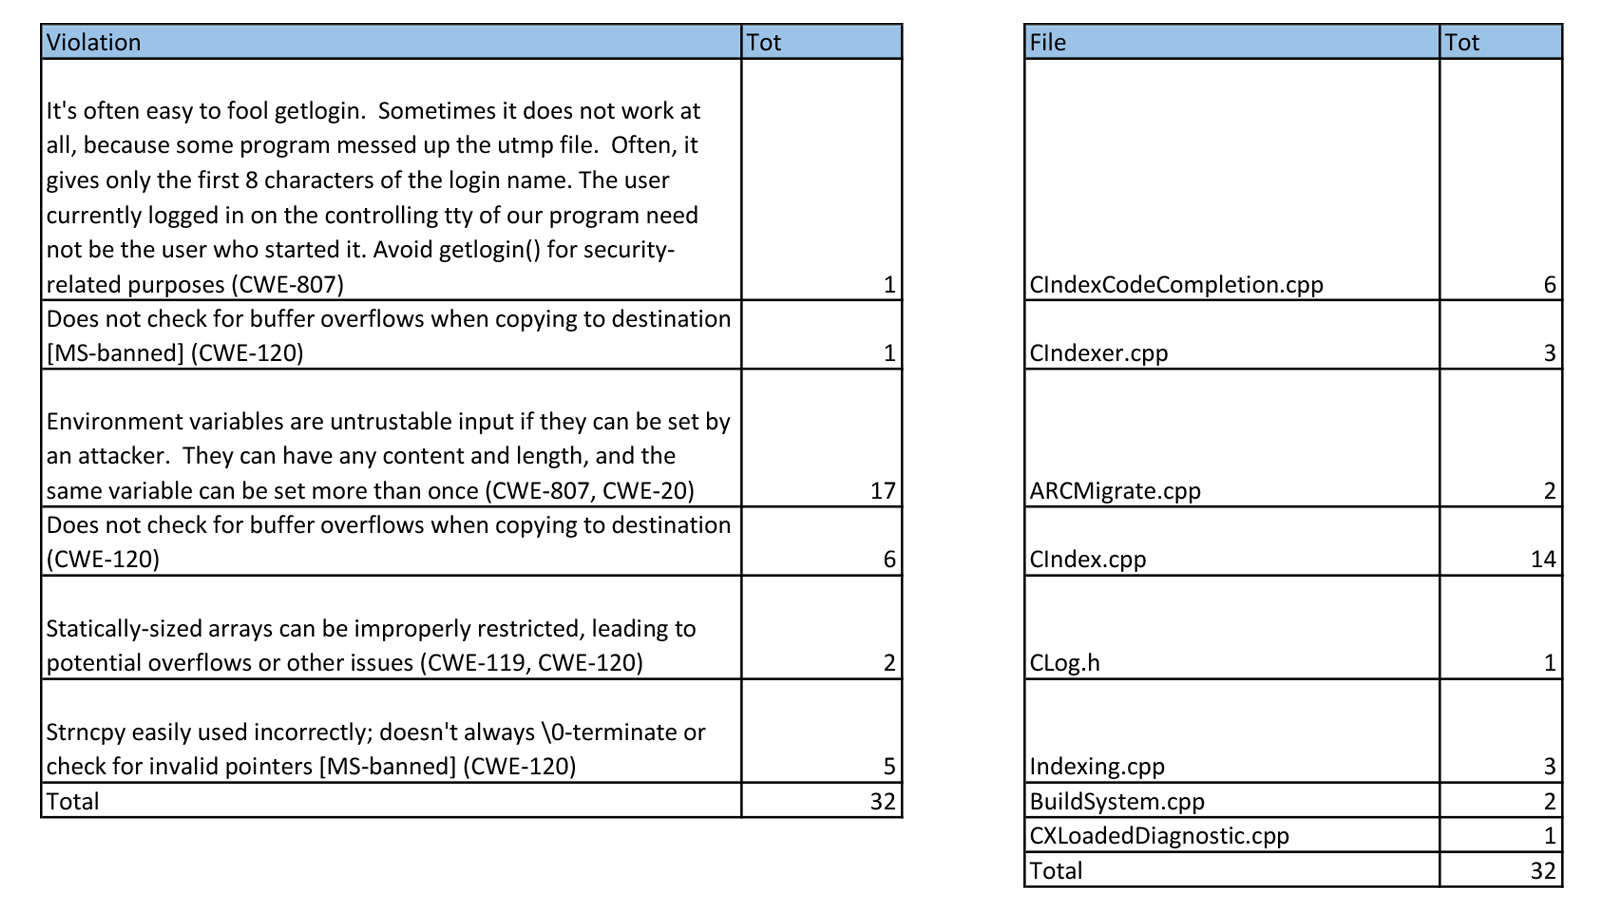
\includegraphics[width=\textwidth]{img/Flawfinder_Summary.jpg}
	\captionof{figure}{Summary of the Flawfinder checks}
\end{minipage}

\pagebreak


\section{SonarQube \& CERT Rosecheckers}

SonarQube is a well known tool for static analysis, capable of detecting both code quality issues (referred as \textsl{Code Smells} and security issuds.\newline
CERT Rosecheckers is a tool that follows the CERT C coding standard to perform it analyses, including CWEs entries and MISRA rules.\newline\newline
These tools were not used in this work since they requires the build of the whole project.

\subsection{SonarQube}

SonarQube (available also via cloud at \url{https://sonarcloud.io}) is a general languages analysis tool. It uses different standards such as MISRA, CERT\dots and it also offers the possibility to define custom rules.\newline
On SonarCloud after an organization's name is defined and a token linked to the project is created, the steps to follow to perform an analysis (on a Linux system) are the following:
\vspace{1cm}

\begin{minipage}{\linewidth}
	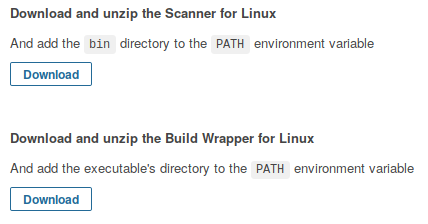
\includegraphics[width=\textwidth]{img/sonarqube-init.png}
	\captionof{figure}{The build-scanner and the build-linux-wrapper have to be downloaded to perform the analysis locally}
\end{minipage}

\begin{minipage}{\linewidth}
	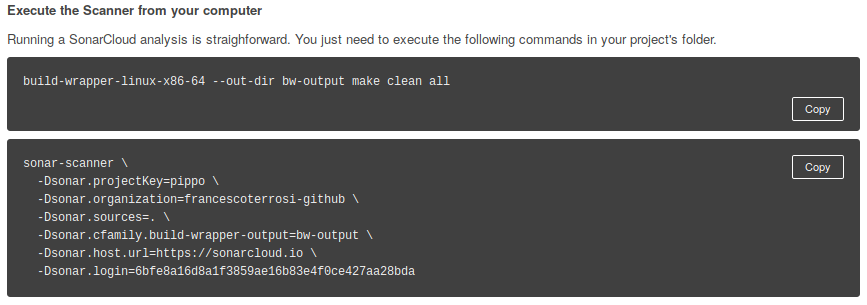
\includegraphics[width=\textwidth]{img/sonarqube-scan.png}
	\captionof{figure}{The first command is used to compile the project.\newline
	The second set of commands is used by SonarQube scanner to scan the project.\newline
	As already mentioned, given the huge size of LLVM-Clang, this was unfeasible}
\end{minipage}

\subsection{CERT Rosechecker}

CERT Rosecheckers is a free tool that can be downloaded from \url{https://sourceforge.net/projects/rosecheckers/} and it is available pre-installed in a Virtual Machine.\newline
Once the virtual machine is executed it is possible to perform the analysis from the shell of the VM. It works by specifying a file, a set of files or a directory:

\begin{itemize}
	\item rosecheckers -rose:[OPTIONS] [FILES/DIRECTORY]
\end{itemize}

\begin{minipage}{\linewidth}
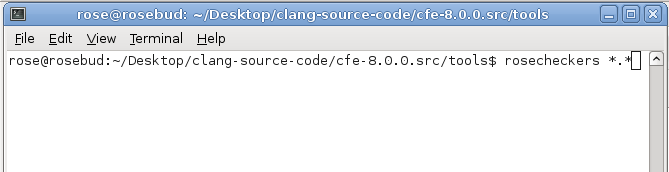
\includegraphics[width=\textwidth]{img/rosechecker-commandline.png}
\captionof{figure}{Screenshot of the Rosechecker Virtual Machine}
\end{minipage}
\pagebreak

Listed below are some of the main options offered by Rosechecker:

\begin{itemize}
	\item \textsl{C\_Only}, \textsl{Fortran}, \textsl{Cxx\_Only} and more to select specific languages source files
	\item \textsl{strict} for a strict enforncement of ANSI/ISO standards
	\item \textsl{excludeCommentsAndDirectives} to exlude comments and preprocessor directives
	\item And more (see rosechekers --help for more informations)
\end{itemize}

The problem with this tool was that it requires all the \textsl{\#include} files to be in the same directory.\newline\newline

\begin{minipage}{\linewidth}
	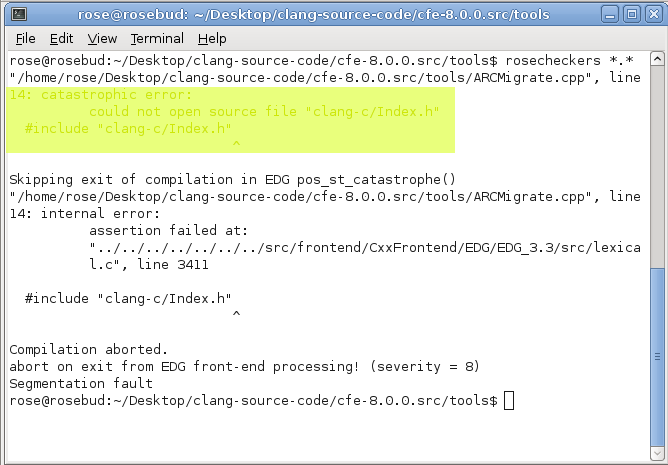
\includegraphics[width=\textwidth]{img/rosechecker-error.png}
	\captionof{figure}{Screenshot of the missing include fatal error}
\end{minipage}
\pagebreak

There are two different solutions for this problem:
\begin{itemize}
	\item Manually remove all the \textsl{\#include} directives from the source files
	\item Manually move all the \textsl{\#include} files in the directory to be analyzed
\end{itemize}

Obviously, the first solution is conceptually incorrect: the analysis is going to be performed on files that have been modified, compromising the final results.\newline
The second approach is more reasonable (even if the project structure is modified we are interested only on a subset of the whole project and, in this way, we are not changing the interested source code files) but \textsl{Rosecheckers} looks in a recursive way for the \textsl{\#include} files in the files to be included, and so on\dots\newline\newline
[e.g.]
\begin{itemize}
	\item CIndex.cpp has the include directive "\#include "clang/AST/Attr.h""
	\item To solve the missing include issue is necessary to copy the \textsl{clang/AST)} directory in the analysis-root folder.
	\item Rosechecker will then check the "include files" of the included file "Attr.h"
	\item Attr.h has the include directive "\#include "clang/AST/Type.h""
	\item To solve the missing include is necessary to to copy the \textsl{clang/AST)} directory in this path: \textsl{analysis-root/clang/AST}
	\item At this point we have this situation: \textsl{analysis-root/clang/AST/clang/AST}
	\item This procedure must be followed to solve all the \textsl{missing include} issues
\end{itemize}

This recursive procedure is obviously unfeasible since the number of folders to be copied/created grows exponentially with respect to the number of files to be included in a single source (or header) file.